% 03-resultados.tex | 3 Results
% RESTAURADO DO ORIGINAL em 06/11/2026: secao 4 do Paper Training - 15 Nov 2025 (4.1 AS9100, 4.2 CAR,
% 4.3 revisao do processo, 4.4 aplicacao dos quatro niveis, 4.4 [sic] impacto no custo da qualidade).
% Edicao: as descricoes longas (clausulas, pilares do SMS, passo a passo do fluxograma, cores das barras)
% foram condensadas sem perder nenhum item; as cores das barras passaram para as notas das figuras.
% Graficos de dados: os ORIGINAIS (Figs. 8 a 10 do original). Os "reconstruidos" da versao JATM
% (valores diferentes dos originais) estao em figs-tikz/_reconstrucoes-jatm-NAO-USAR/.
% Correcao: o original dizia "Figure 8 reveals that the average score for the 21 employees was 66.90";
% a media e da Fig. 9 do original (aqui Fig. 7).
% Da versao JATM: so o paragrafo de traducao para sustentabilidade (3.5), que nao conflita.

\section{Results}
\label{sec:results}

\subsection{AS9100 training requirements}
\label{subsec:as9100}

The review of the \AS{} standard identified the clauses pertinent to training and risk management, highlighted in green in Figure~\ref{fig:as9100}. Actions for risks and opportunities (clause 6.1) require the organization to identify and address risks and opportunities through planned actions. Resources (7.1) require enough qualified personnel for the quality management system and its processes. They also require the organization to define, preserve and make available the knowledge needed for process execution and product conformity, using existing knowledge, acquiring expertise and incorporating updates as demands evolve. Organizational knowledge comprises institution-specific insight from experience, intellectual property, lessons learned, undocumented expertise and improvements in processes, products and services, supplemented by standards, academia, conferences, customers and external providers. Competence (7.2) requires the organization to determine the competence of people whose work affects the performance of the quality management system, to ensure it through education, training or experience, to act to improve skills, to evaluate the effectiveness of those actions and to retain documented evidence. Periodic competence reviews may lead to training, mentoring, reassignment, or hiring and contracting competent people. Awareness (7.3) requires employees to know the quality policy, the relevant objectives and their contribution to the effectiveness of the system. This includes the benefits of improved performance, the implications of non-conformance, the relevant documented information and its changes, and their contribution to product and service conformity, safety and ethical conduct. Communication (7.4) requires protocols for internal and external communication about the quality management system, defining what is communicated, when, to whom, how and by whom. Finally, operational risk management (8.1.1) requires a structured process to plan, implement and control operational risks to the organization, products and services. The process assigns responsibilities and defines risk assessment criteria; risks are identified, analyzed and communicated, those above the acceptance threshold are mitigated, and residual risks are accepted after mitigation.

\begin{figure}[H]
  \centering
  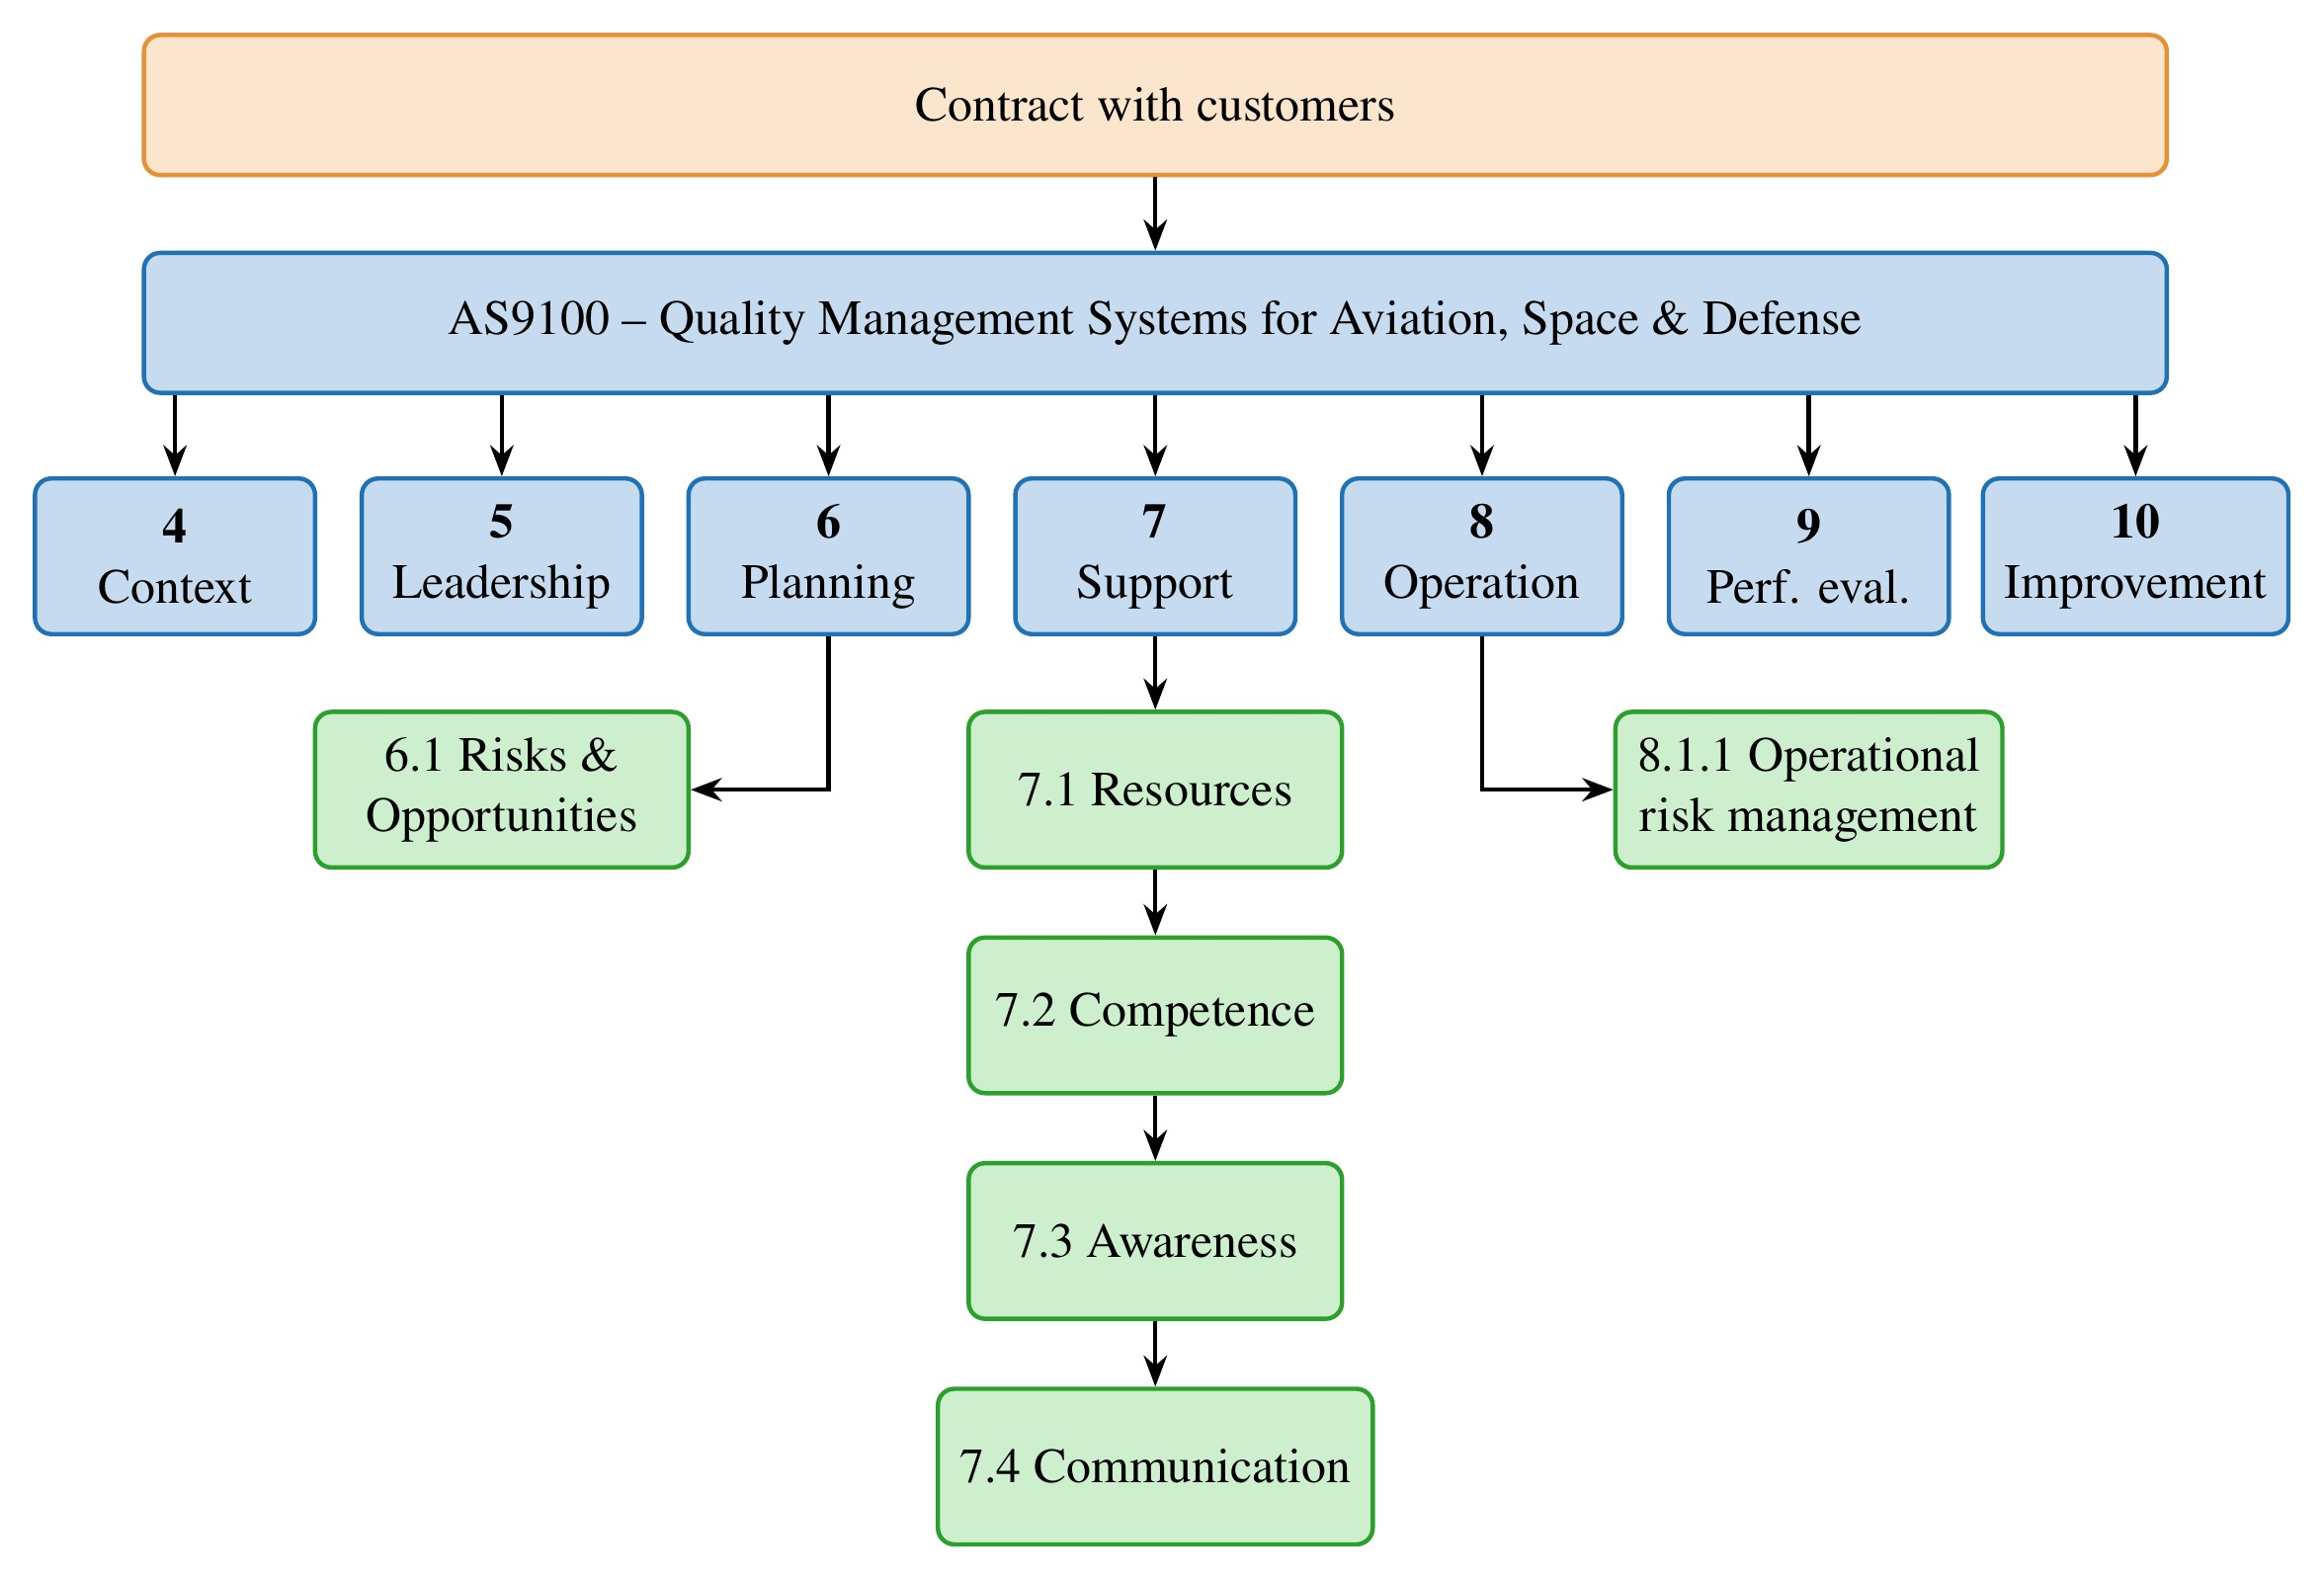
\includegraphics[width=0.9\linewidth]{fig2-as9100}
  \caption{AS9100 requirements relevant to maintenance training}
  \label{fig:as9100}
  \notafonte{Clauses relevant to training are highlighted in green. AS9100: Quality Management Systems, Requirements for Aviation, Space and Defense Organizations. Source: the authors, based on the AS9100 standard.}
\end{figure}

\subsection{Civil aviation regulation training requirements}
\label{subsec:car}

The civil aviation regulation (CAR) requirements applicable to repair stations were examined to delineate specific training mandates (Figure~\ref{fig:regulation}). The framework descends from the International Civil Aviation Organization (\ICAO{}) to civil aviation authorities (for example, \FAA{}, \EASA{} and \ANAC{}) and on to airlines, airports and maintenance facilities (repair stations). Certificated repair stations must implement an authority-accepted employee training program, with initial and recurrent training. Applicants for a repair station certificate must submit a training program for approval, ensuring that employees who perform maintenance, preventive maintenance, alterations and inspections are adequately trained. Repair stations must also keep detailed, authority-approved records of each employee's training. Training duties also run through the four \SMS{} pillars. Safety policy, objectives and procedures set duties, accountabilities and safety objectives, with a safety manual of policies, compliance procedures, instructions for safety-related activities (management controls, documentation, corrective actions) and alignment with the authority's safety management. Safety risk management requires hazard identification, risk controls, agreed acceptable safety performance, risk owners and controlled mitigation, with a data-driven choice of safety indicators, targets and surveillance priorities. Safety assurance relies on oversight and surveillance: systematic collection, analysis and sharing of safety data, risk-based surveillance, safety system audits, management of change and continuous improvement, including investigations and root cause analyses. Safety promotion builds safety culture through training, communication and two-way dissemination of safety information. \SMS{} training targets safety specialists, leadership and staff, including the inspectors responsible for \SMS{} acceptance and safety performance; it evolves continuously, with documented \SMS{} procedures as the basis for communication and stakeholder feedback.

\begin{figure}[H]
  \centering
  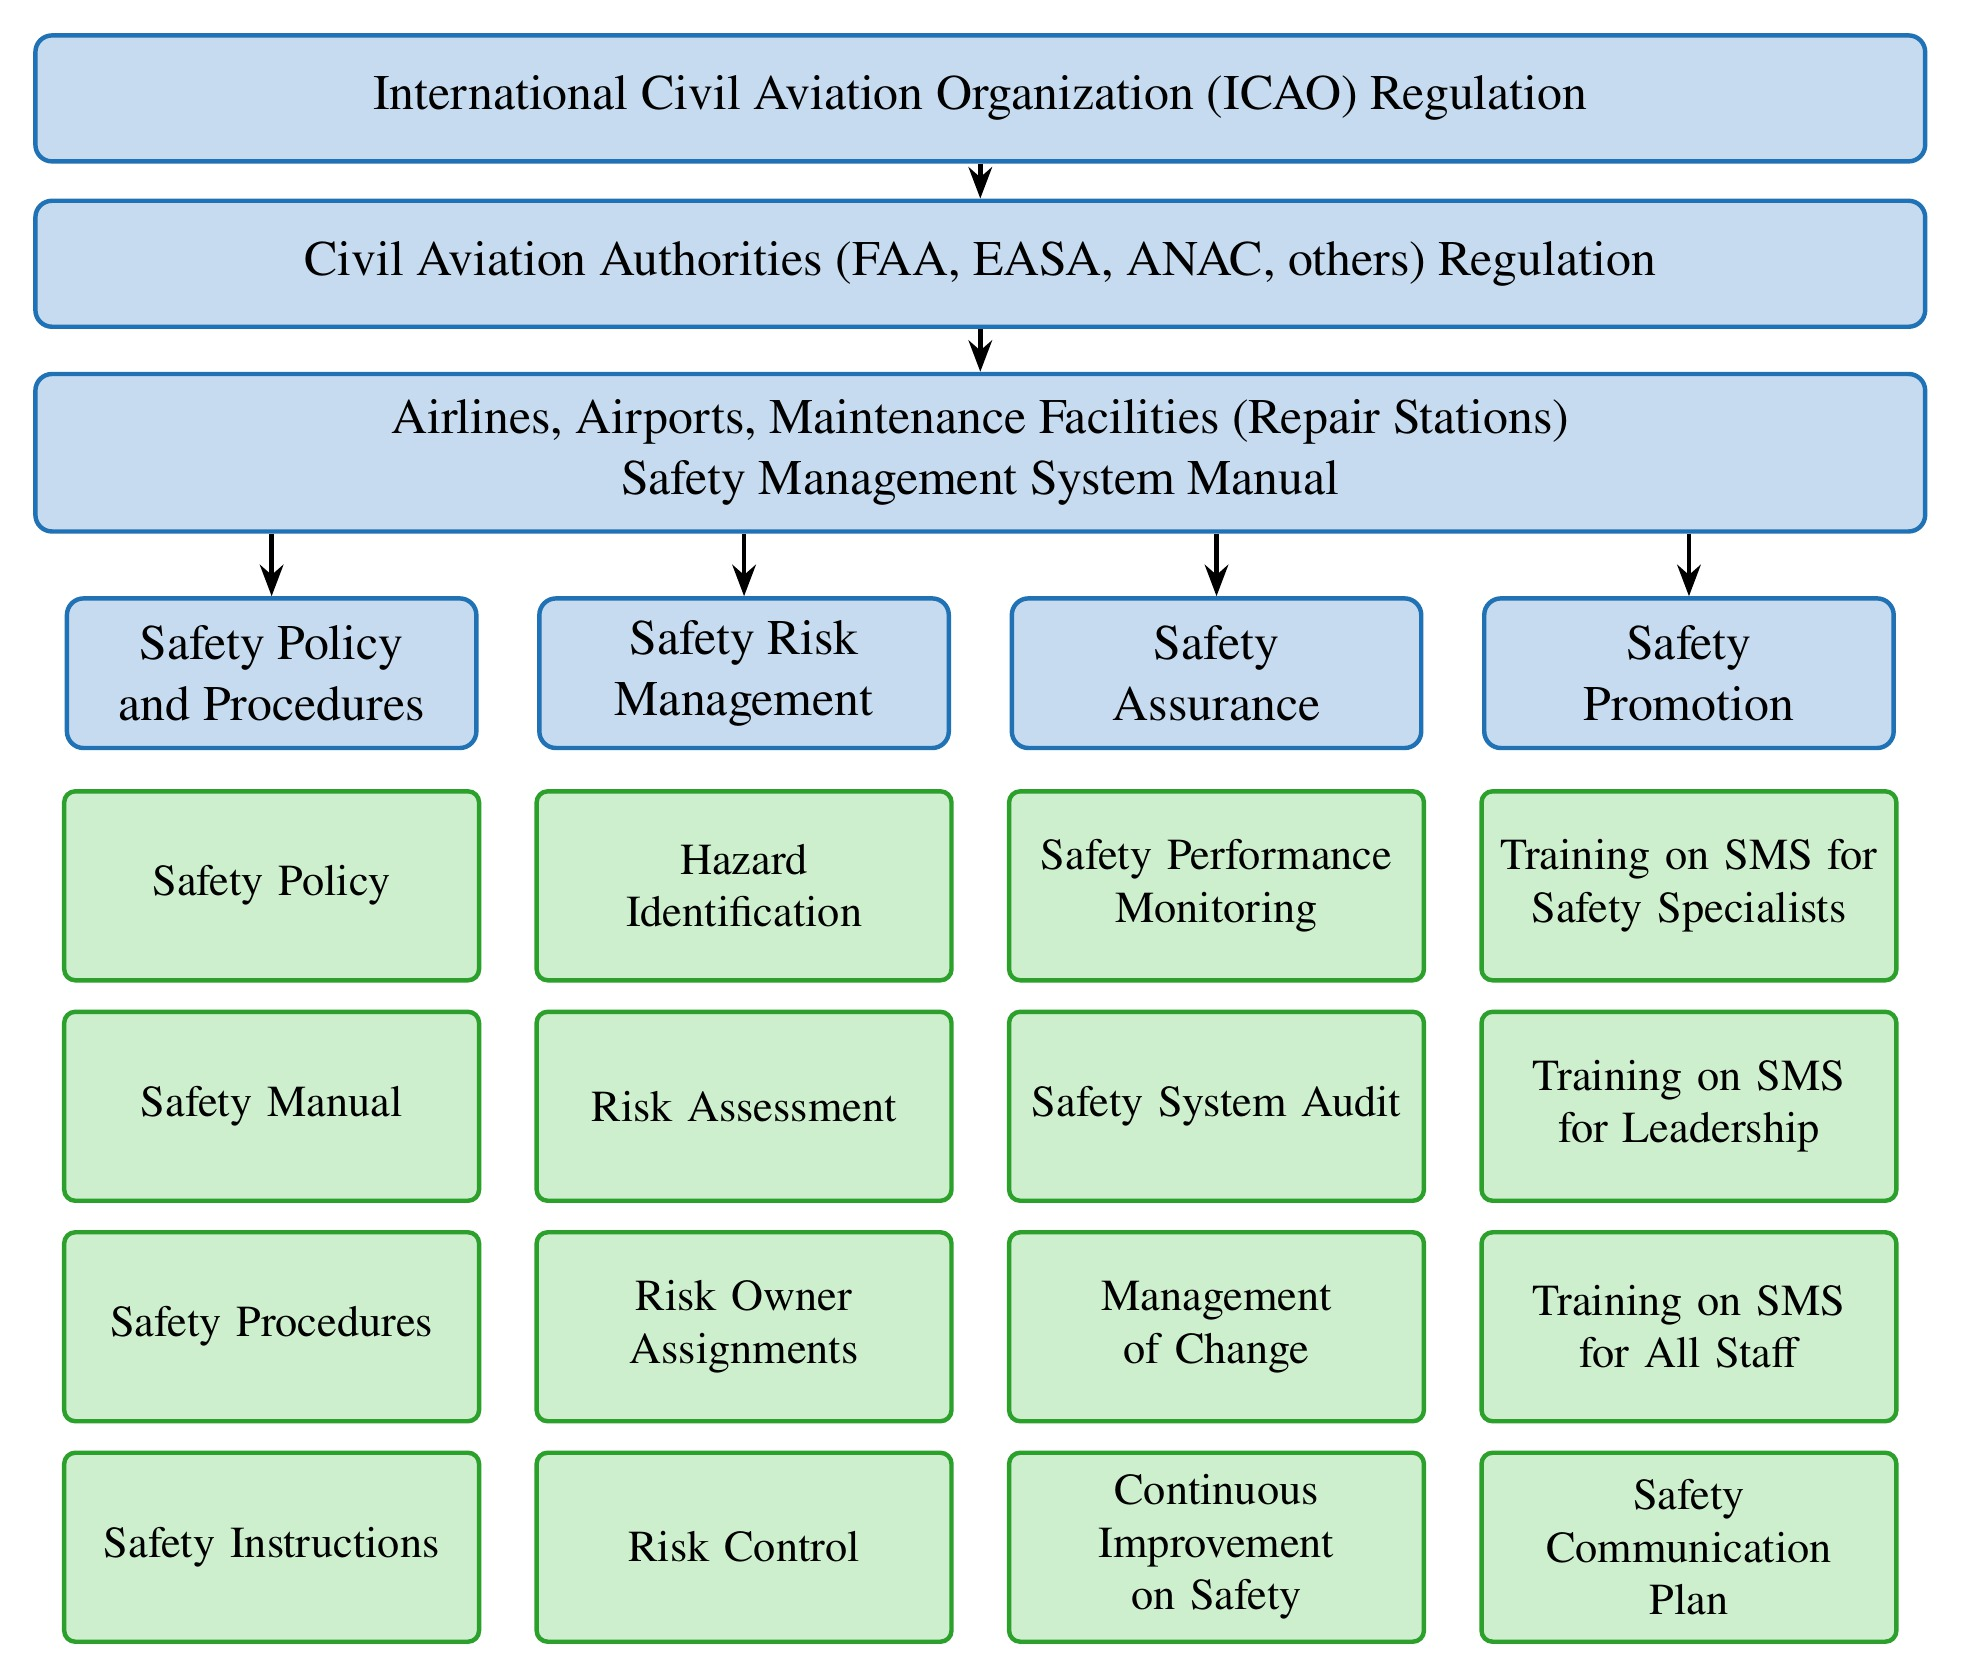
\includegraphics[width=0.9\linewidth]{fig3-regulation}
  \caption{Regulatory cascade and SMS components}
  \label{fig:regulation}
  \notafonte{SMS components in green. ICAO: International Civil Aviation Organization; FAA: Federal Aviation Administration; EASA: European Union Aviation Safety Agency; ANAC: Brazilian National Civil Aviation Agency; SMS: Safety Management System. Source: the authors, based on ICAO and civil aviation authority regulations.}
\end{figure}

\subsection{Aircraft engine maintenance training management process}
\label{subsec:process}

The case focused on the training program of the facility's Technical Training Area, which oversees more than 50 distinct courses and delivers an average of 30,000 training hours a year to develop employees' technical expertise and performance. Because it directly influences product and service quality, the area operates under quality management. The study validated organizational tools at each Kirkpatrick level, with distinct methods and follow-up actions: a tailored questionnaire for reaction, final grades for learning, dual questionnaires (trainees and supervisors) for behavior, and customer satisfaction data from quality management for results. All questionnaires followed a semi-structured script derived from the literature review, and pre- and post-assessment analyses were used to examine the role of the evaluation as a continuous improvement instrument. The training management process covers the planning, resourcing, delivery, demonstration and measurement of technical training and its curriculum, delivered by qualified instructors (Figure~\ref{fig:process-original}). It runs from the identification of training needs (organizational goals, skill gaps, regulatory requirements) to the archiving of records for reference, compliance and audit. Two systems support it: the learning management system (\LMS{}), which holds classes, attendance, grades and certificates, and the enterprise resource planning (\ERP{}) system, to which only trained employees are given access.

\begin{figure}[H]
  \centering
  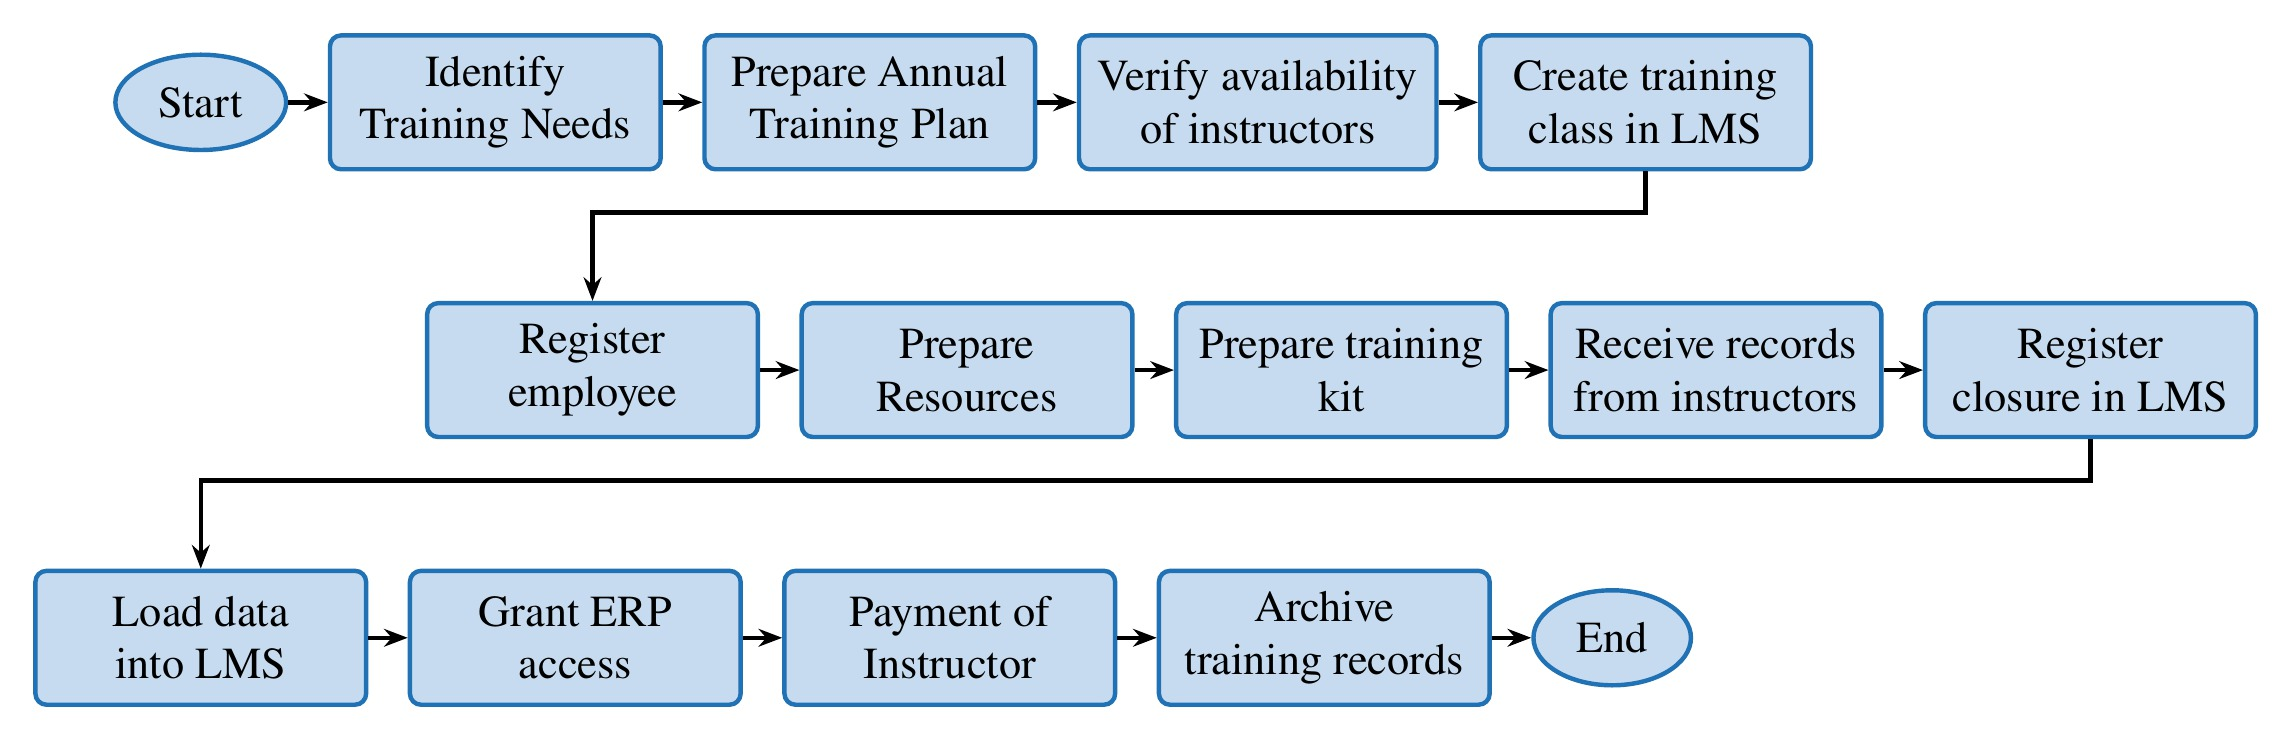
\includegraphics[width=0.9\linewidth]{fig4-process-original}
  \caption{Order of activities in the training process}
  \label{fig:process-original}
  \notafonte{LMS: learning management system; ERP: enterprise resource planning. Source: the authors.}
\end{figure}

Reaction evaluation already existed in the company but was done manually, which prompted the first improvement. A functional flowchart revealed bottlenecks and waste: excessive processing, long waits between operations and an overload of documents to archive. An online questionnaire, built with company-approved software and informed by the literature, replaced the paper form. Instructors send its link to trainees at the end of each session, and the software keeps a response database and generates the metrics automatically. The questionnaire gauges trainees' opinion of and satisfaction with the knowledge acquired, the materials, the room infrastructure, the content and the instructor's methodology. The 5W2H tool was used to map each activity. The revised process (Figure~\ref{fig:process-redesigned}) adds the reaction, learning, behavior and results evaluations at the end of the original flow. It does so in three new activities: evaluation of the four levels, verification of the data for each level and data-based optimization of training. Regular employee feedback shows whether training works and how it is received. For job-specific training, productivity, production and quality before and after training measure efficacy, and the training plan is modified and expanded as the company grows. The revised process was designed to strengthen training effectiveness and so mitigate the risk of training deficiencies and of the operational failures that stem from inadequate preparation.

\begin{figure}[H]
  \centering
  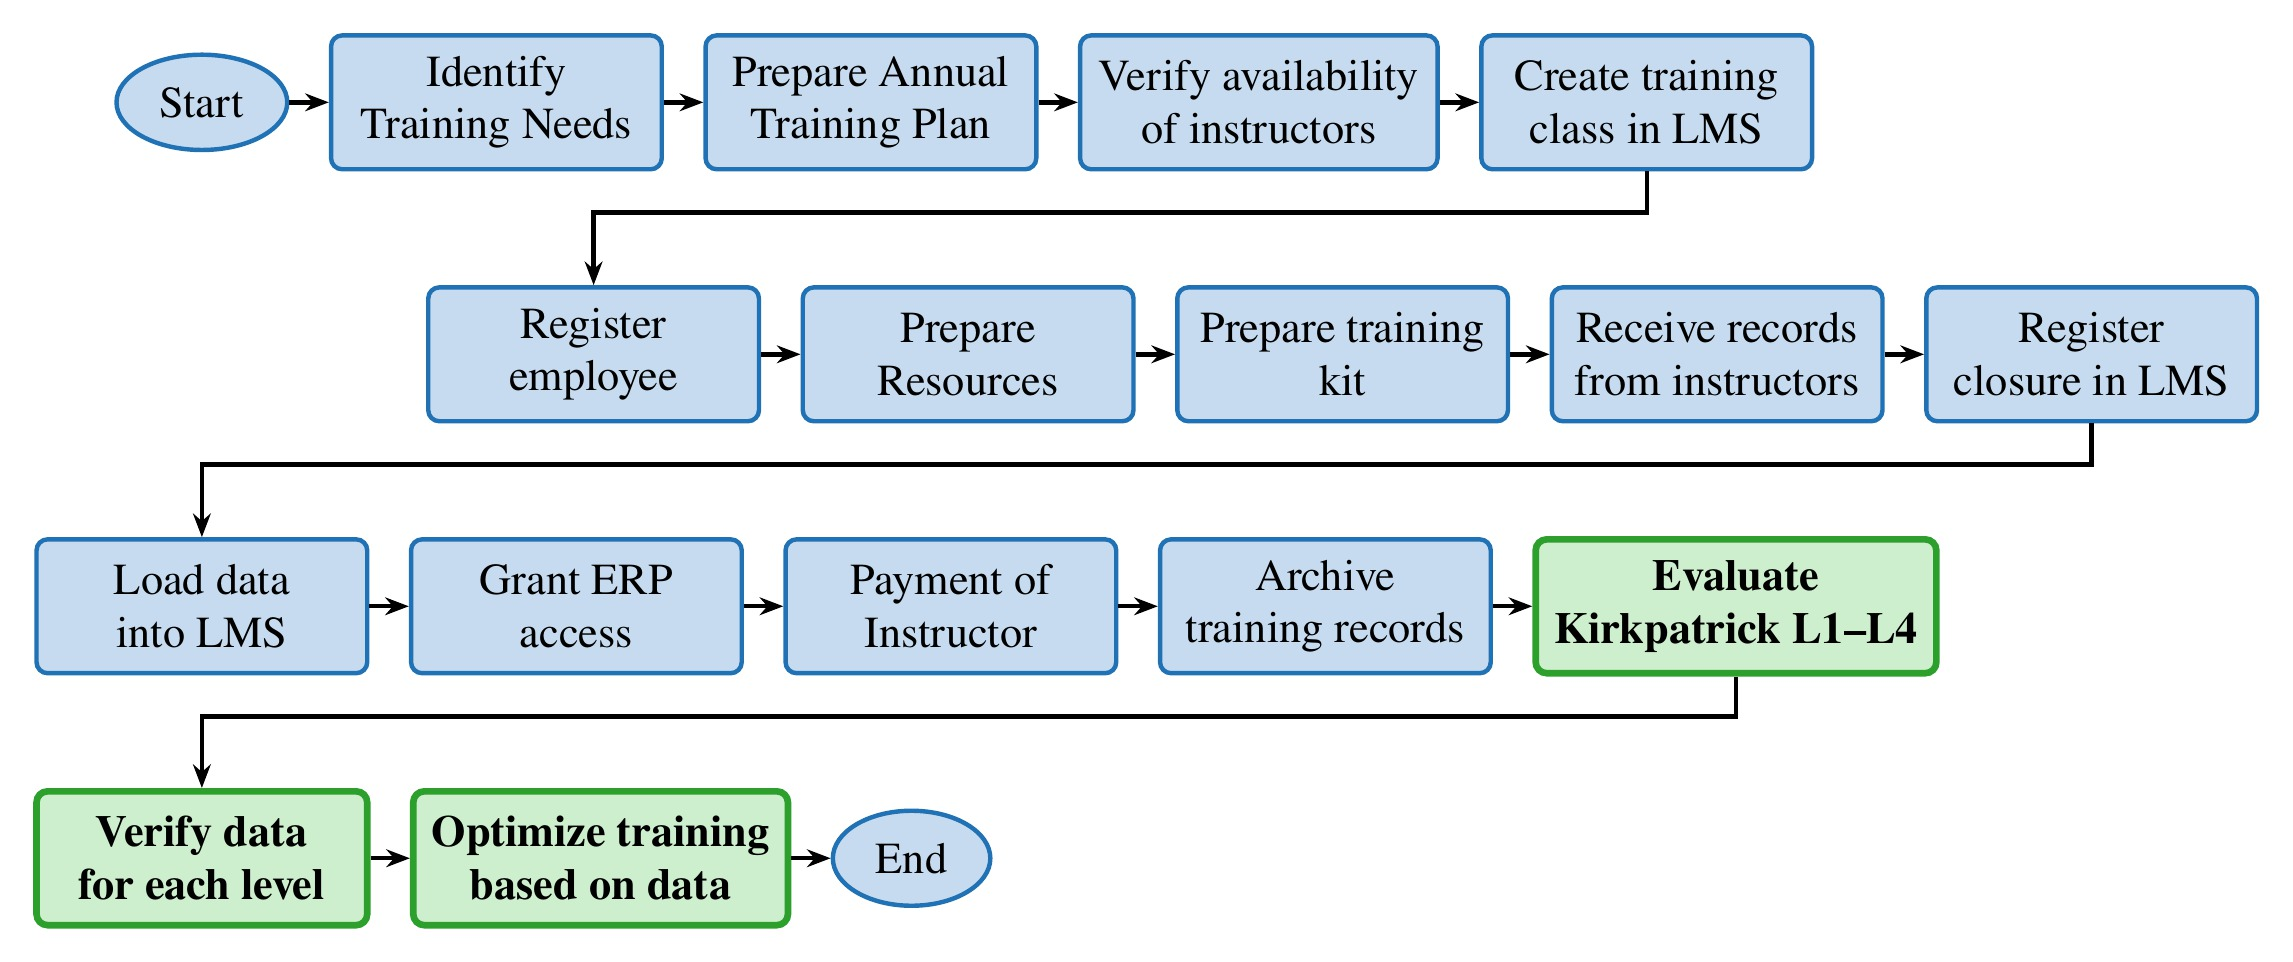
\includegraphics[width=0.9\linewidth]{fig5-process-redesigned}
  \caption{Order of activities in the training process after the change}
  \label{fig:process-redesigned}
  \notafonte{New activities in green. LMS: learning management system; ERP: enterprise resource planning. Source: the authors.}
\end{figure}

\subsection{Application of Kirkpatrick's four levels}
\label{subsec:levels}

\textbf{Level~1, reaction.} Using the software-generated results, the study analyzed the average score of each question across sessions, producing metrics for learning, satisfaction, content, punctuality, communication, mastery and infrastructure. Figure~\ref{fig:scores-reaction} shows a sample of ten sessions. Most scores were close to 10 on the 0--10 scale; content scored about 5 and 4 in two sessions and infrastructure below 8 in another, the content and infrastructure gaps discussed in Section~\ref{subsec:disc-reaction}.

\begin{figure}[H]
  \centering
  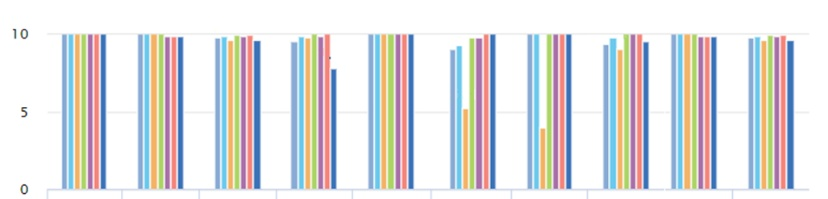
\includegraphics[width=0.9\linewidth]{fig6-reaction-scores}
  \caption{Sample of the reaction scores from ten training sessions}
  \label{fig:scores-reaction}
  \notafonte{Groups from left to right: sessions 1 to 10. Bars in each group, from left to right: learning, satisfaction, content (orange), punctuality, communication, mastery and infrastructure. Scale from 0 to 10. Source: facility training records (original chart). \todo{imagem original a 115 dpi; a revista pede 300 dpi ou mais: pedir ao autor correspondente o gráfico ou a planilha de origem}}
\end{figure}

\textbf{Level~2, learning.} The Training Area's existing tools were used: a test at the end of each session verifies the trainees' learning. The average score of the 21 trainees was 66.90 out of 100 (Figure~\ref{fig:scores-grades}), below the pass mark of 70, with at least seven trainees below it. The data analysis therefore pointed to the need to improve the learning assessment, and the Training Area representative met the instructors to review the content and make it clearer and more accessible to employees.

\begin{figure}[H]
  \centering
  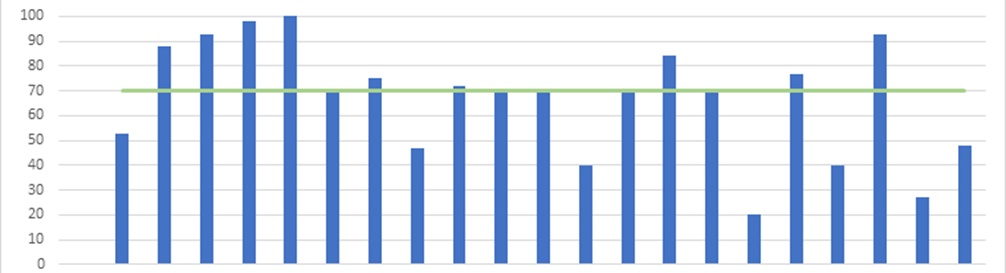
\includegraphics[width=0.9\linewidth]{fig7-final-grades}
  \caption{Final grades of 21 trainees}
  \label{fig:scores-grades}
  \notafonte{Blue bars: individual grades on a 0--100 scale; green line: minimum passing grade (70). Source: facility training records (original chart). \todo{imagem original a 137 dpi; pedir o gráfico ou a planilha de origem}}
\end{figure}

\textbf{Level~3, behavior.} A dual questionnaire answered by trainees and their leaders checked whether behavioral changes emerged months after training and whether the knowledge lasted. A 5W2H analysis set objectives and responsibilities for this and the other levels. For employees, the questionnaire was a self-assessment of the training's effect on their work environment, post-training errors, behavioral changes and their sense of encouragement after the course. Leaders answered parallel questions on the trained employees' performance. Both questionnaires used the same software as the reaction evaluation, which generated data and charts for each item. The effectiveness threshold was an average of 70 on a 0--100 scale. Scores below it for work area, acquired knowledge or behavioral change trigger an investigation of the training's relevance to the employee's role or of content updates for area-specific demands. \todo{o original não traz os resultados do Nível 3 (médias das 15 duplas por item); incluir}

\textbf{Level~4, results.} External customer satisfaction was evaluated in the first months of the study year on a 0--5 scale (0, very dissatisfied; 3, neutral; 5, very satisfied). The categories were product delivery quality, availability of technical documentation, turnaround time (TAT), customer support and engineering team assistance. Figure~\ref{fig:customer-satisfaction} shows the ratings of the four customers, all between 3 and 5; the ratings of 3 concerned technical documentation and turnaround time. After the quarterly review, scores below 3 trigger a detailed investigation of the items critical to customers and of improvement opportunities through technical training, either by revising existing programs or by developing new material. Table~\ref{tab:results-by-level} summarizes the results by level.

\begin{figure}[H]
  \centering
  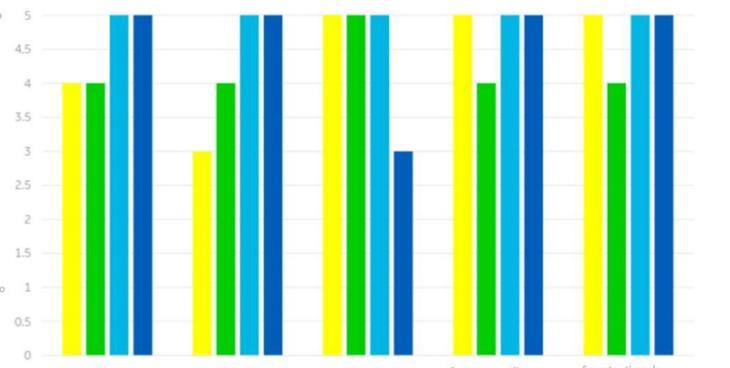
\includegraphics[width=0.75\linewidth]{fig8-customer-satisfaction}
  \caption{Customer satisfaction per category}
  \label{fig:customer-satisfaction}
  \notafonte{Groups from left to right: product delivery quality, quality of technical documentation, turnaround time, customer support and engineering team support. Bars: client 1 (yellow), client 2 (green), client 3 (light blue) and client 4 (dark blue). Scale from 0 (very dissatisfied) to 5 (very satisfied). Source: facility customer surveys (original chart). \todo{imagem original a 164 dpi; pedir o gráfico ou a planilha de origem}}
\end{figure}

% Tabela 1 | Resultados por nivel, SO com numeros do artigo original (Paper Training - 15 Nov 2025):
% secoes 2.5, 3.2 e 4.4 do original e os graficos originais (Figs. 8 a 10 do original = Figs. 6 a 8 aqui).
% "Pelo menos sete abaixo de 70" e "notas de 3 a 5" foram lidos dos graficos originais; a leitura da
% Fig. 9 confere com a media de 66,90 do texto original (soma 1.405 / 21).
\begin{table}[H]
  \centering
  \caption{Results of the Kirkpatrick-based evaluation by level}
  \label{tab:results-by-level}
  \footnotesize
  \begin{tabularx}{\linewidth}{@{}>{\raggedright\arraybackslash}p{2.6cm} >{\raggedright\arraybackslash}p{4.2cm} >{\raggedright\arraybackslash}X@{}}
    \toprule
    \textbf{Level} & \textbf{Instrument and sample} & \textbf{Result and action} \\
    \midrule
    L1 Reaction & Online questionnaire, seven criteria, 0--10 scale; 10 sessions & Most scores close to 10; content scored about 5 and 4 in two sessions and infrastructure below 8 in one; items below target were followed up \\
    \addlinespace
    L2 Learning & End-of-session test, pass mark 70/100; 21 trainees & Mean 66.90; at least seven trainees below the pass mark; content reviewed with instructors \\
    \addlinespace
    L3 Behavior & Dual questionnaires (trainee and leader), 3 to 12 months after training; 15 pairs & Threshold 70/100; scores below it trigger investigation of relevance or content \\
    \addlinespace
    L4 Results & Customer survey, five categories, 0--5 scale; four airline customers & Ratings between 3 and 5; the ratings of 3 concerned technical documentation and turnaround time \\
    \addlinespace
    Organizational outcomes & Quality management system and quality-cost records; twelve months & 28\% fewer training failures; 35\% fewer regulatory non-conformances; quality costs about USD 1.2 million a year lower \\
    \bottomrule
  \end{tabularx}
  \notafonte{L1 to L4: Kirkpatrick levels. Source: the authors, from the facility's training, quality and customer records. \todo{F2: resultado do Nível 3 (médias das 15 duplas) e contagens que sustentam 28\% e 35\%}}
\end{table}


\subsection{Impact of ineffective training on costs of quality}
\label{subsec:coq}

Historical data and the literature show that \MRO{} companies face a costly cycle of quality issues rooted in ineffective training. The cycle includes material loss from scrapped components, rework that consumes additional labor and materials, test-cell rejections that require fuel-consuming re-tests, and warranties or concessions that demand further repairs at the customer site or in-house, often with round-the-clock effort and expedited shipping. The cycle persists when inadequately trained employees, lacking skill-based competence and the situational awareness to grasp the criticality of their actions, become disengaged and less careful with safety and quality protocols. Their errors become more frequent, and a safety-escape management system weakened by a lack of root-cause-analysis training tracks and investigates them poorly. Superficial corrective actions then let the gaps persist and the same non-conformances recur. Quality costs (prevention, appraisal and failure) escalate and the safety margin erodes, raising the risk of a catastrophic operational failure. Cost estimates from detailed non-conformance investigations show how a single lapse can trigger a chain of repercussions. Two examples are improper handling training that leads to damage of a high-value high-pressure turbine (HPT) stage 1 disk, and incorrect assembly training on an oil pump that results in an in-flight shutdown and subsequent engine rejection. \todo{dizer se o disco HPT e o desligamento em voo são casos da instalação (com a estimativa de custo) ou ilustrações; e dar fonte para ``historical data and the literature show''} Thorough, effective and engaging training across all critical \MRO{} functions, from receiving inspection and powerplant disassembly to non-destructive testing and adherence to aviation regulations, is therefore the primary defense against both financial loss and safety catastrophe.

Over the twelve months of the intervention, training failures fell by 28\%, regulatory non-conformances by 35\% and quality costs by about USD~1.2 million a year (Section~\ref{subsec:bridge}). \todo{F2: as contagens e a decomposição do custo pelo modelo da seção 2.5} Managers reported 92\% satisfaction with the framework's audit readiness, noting that it ``transformed training into a measurable asset'' (focus group, 2025). The methodology can be applied beyond aviation, for example to manufacturing under similar standards, by adapting Kirkpatrick to local regulations. It also opens research directions such as cross-industry validation and machine learning for real-time Level~4 prediction. In sustainability terms, the reductions in scrap, rework and expedited shipping imply lower material consumption, energy use and transport emissions. Every component not scrapped preserves its embodied energy and raw material, and every overhaul not reworked preserves the corresponding labor hours and facility energy. Quantifying these effects in kilograms, kilowatt-hours and kgCO\textsubscript{2}e is left to future work.
